\documentclass[12pt]{article}
\usepackage{amsmath}
\usepackage{jheppub}

\newcommand{\IGNORE}[1]{}
\newcommand{\be}{\begin{equation}}
\newcommand{\ee}{\end{equation}}
\newcommand{\bea}{\begin{aligned}}
\newcommand{\eea}{\end{aligned}}

\title{Gibbons-Hawking-York Boundary Term in Causal Sets}
 \author[a]{M. Buck}
 \author[a,b]{\!, F. Dowker}
 \author[a]{and I. Jubb\,}
\affiliation[a]{Theoretical Physics Group, Blackett Laboratory, Imperial College, London, SW7 2AZ, U.K.}
\affiliation[b]{Institute for Quantum Computing, University of Waterloo, ON, N2L 2Y5, Canada}

\abstract{ 
We show some stuff.
}

\begin{document}

\maketitle


\noindent NOTES:\\
1. define s as the RV, not as its mean

\section{Introduction}

%[MB1: USEFUL QUOTE FROM RAFAEL: In the quantum theory, however, these boundary terms are important. They are essential in order that the quantum mechanical amplitudes satisfy the correct composition law and in order that these amplitudes have the correct classical limit. In a number of examples [5] they give a contribution to the partition function which is important for the agreement with calculations based on straightforward thermo- dynamics. In this note we shall derive the boundary terms in the action for the Regge calculus]

In furthering causal set theory it is crucial that we understand the kinematics of the theory. The action of a given causal set is a crucial piece of the kinematics that would be extremely useful to know and understand. Proposals for the action of a causal set are available \cite{Benincasa_Dowker:The_Scalar_Curvature_of_a_Causal_Set} and these hold analytically in some cases and numerically in many more. These cases being when the causal set is embeddable in some existing spacetime. One can show that the action of the causal set then agrees with the Einstein-Hilbert (EH) action of the spacetime in some continuum limit. How this limiting procedure is carried out will be described in more detail below.

The EH action, however, is not the complete story in the continuum. If one has a spacetime manifold with a boundary, such as Minkowski space but cut off at some finite time, then one needs to include the Gibbons-Hawking-York boundary term (GHYBT) in the EH action \cite{Gibbons_Hawking_Boundary}. The boundary of the manifold will be some hypersurface of codimension-1. The GHYBT is an integral over this hypersurface, of the extrinsic curvature that it has. This term is needed in the action to keep the variational principle well defined. In this paper we turn our attention to this term, and provide the causal set analogue for spacelike hypersurfaces.

We define a \textit{causal set} (or \textit{causet}) as a locally finite partial order. This means it is a pair $(\mathcal{C},\preceq)$ where $\mathcal{C}$ is the set of points and $\preceq$ is a partial order relation on $\mathcal{C}$ that has the following properties. It is (i) reflexive: $x\preceq x$, (ii) acyclic: $x\preceq y\preceq x \Rightarrow x=y$, and (iii) transitive: $x\preceq y\preceq z \Rightarrow x\preceq z$ for all points $x, y, z \in \mathcal{C}$. We define an inclusive order interval as the set $I(x,y):=\lbrace z\in\mathcal{C}|x\preceq z\preceq y\rbrace$ for any $x, y\in\mathcal{C}$. The \textit{locally finite} condition is simply that the cardinality of any order interval is finite, that is $|I(x,y)|<\infty$. This condition ensures we are dealing with a discrete structure, as all the other properties of the relation would apply to an order relation between points on a continuous manifold.

In order to say we have a causal set analogue for a continuous expression we need a well defined procedure for relating the discrete theory to the continuum. This procedure, or tool, is called a \textit{Poisson sprinkling}, or just a \textit{sprinkling}. It is a Poisson process which provides a way to generate a causet from a $d$-dimensional Lorentzian manifold $(\mathcal{M},g)$ by selecting points in $\mathcal{M}$ to be the elements of $\mathcal{C}$, with an order relation given by the causal order of the manifold. The number of points chosen in a region of spacetime volume, $V$, is a Poisson random variable. This means that the expected number of points in some region will be $\rho V$, where $\rho$ is the density of the sprinkling. The density is related to the discreteness scale, $l$, by $\rho=l^{-d}$ in $d$ spacetime dimensions. It is called a sprinkling as one can envisage the point selection process as a 'sprinkling' of points into the manifold. If a causet, $\mathcal{C}$, can be generated with relatively high probability by a sprinkling into the manifold, $(\mathcal{M},g)$, then we say that the manifold is a good approximation for the causal set.

\section{The Claim}

Consider a sufficiently well-behaved $d$-dimensional spacetime $(M,g)$ and Cauchy surface $\Sigma$ in $M$. The causal past and future sets $M^\pm=J^\pm(\Sigma)$ form a partition of $M$ and $\partial M^\pm = \Sigma$. The Gibbons-Hawking-York boundary term for $M^\pm$ is in this case given by
\be\label{eq:GHYBT_in_continuum}
S_{GHY} = \pm \frac{1}{l_p^{d-2}}\int_{\Sigma} d^{d-1}x \sqrt{h} K
\ee
where $l_p$ is the rationalised Planck length and $K$ is the trace of the extrinsic curvature $K_{\mu\nu}=h_{\mu}^\rho h_\nu^\sigma \nabla_\rho n_\sigma$ of $\Sigma$ defined with future-pointing timelike unit normal $n_{\mu}=\partial_\mu S/\sqrt{g^{\mu\nu}\partial_\mu S\partial_\nu S}$. 

The extrinsic curvature of a spacelike hypersurface can be identified with the volume gradient across that hypersurface [MB1: HOW SO?]. On the causal set, the analogue of a spacelike hypersurface is a maximal anti-chain, i.e. a subset $\mathcal{A}\subseteq\mathcal{C}$ in which all elements are unrelated. These unrelated elements are maximal in the sense that there exist no elements $y\in\mathcal{C}\setminus\mathcal{A}$ such that $x\preceq y$, $\forall x\in\mathcal{A}$. The intuitive analogue of the boundary term would then be the rate of change of the number of causal set elements below and above the antichain. We shall see that this intuitive idea indeed bears out.

Consider a causal set $\mathcal C$ obtained by a Poisson sprinkling at density $\rho=1/l^d$ into a $d$-dimensional spacetime $(M,g)$. A Cauchy surface $\Sigma\subset M$ induces a partition $\mathcal C = \mathcal C^+ \cup\, \mathcal C^-$ of the sprinkling, where $\mathcal C^\pm$ denotes the restriction of $\mathcal C$ to the points sprinkled to the causal future/past of $\Sigma$. Let us denote the number of maximal elements in $\mathcal C^-$ and the number of minimal elements in $\mathcal C^+$ by $N_{max}$ and $N_{min}$, respectively. We propose the following definition for the discrete Gibbons-Hawking-York boundary term:
\be\label{GH_boundary_to_causet}
S^{(d)}_{GHY}[\mathcal C]=\left(l/l_p\right)^{d-2}c_{d}(N_{max}-N_{min})
\ee
where the constant $c_{d}$ only depends on the spacetime dimension and is given by
\be\label{Cn}
c_{d}=\frac{d(d+1)}{2(d+2)\Gamma\left(\frac{2}{d}\right)}\left[\frac{A_{d-2}}{d(d-1)}\right]^{\frac{2}{d}},
\ee
$A_d$ denoting the volume of the unit $d$-sphere. To support this proposal we show that in the limit of infinite sprinkling density into a $d$-dimensional spacetime we obtain
\be
\lim_{\rho\rightarrow\infty}\left\langle S^{(d)}_{GHY}[\mathcal C] \right\rangle= \frac{1}{l_p^{d-2}}\int_{\Sigma} d^{d-1}x \sqrt{h} K\label{eq:mainconjecture}
\ee
where $\left\langle\cdot\right\rangle$ denotes the mean over sprinklings. The limit $\rho\rightarrow\infty$ is equivalent to setting the discreteness scale to zero, $l\rightarrow 0$. Figure \ref{fig:Nmin_Nmax} shows an illustration of the idea behind this conjecture. The minimal and maximal elements have been highlighted and the shaded regions correspond to the regions whose volumes expressions will be needed in the proof.
%MB1: (too vague) During the calculation approximations will be made. These approximations are justified on the grounds that if certain orders are retained throughout the calculation they will in fact vanish in the limit $\rho \rightarrow \infty$
\begin{figure}
  \centering
    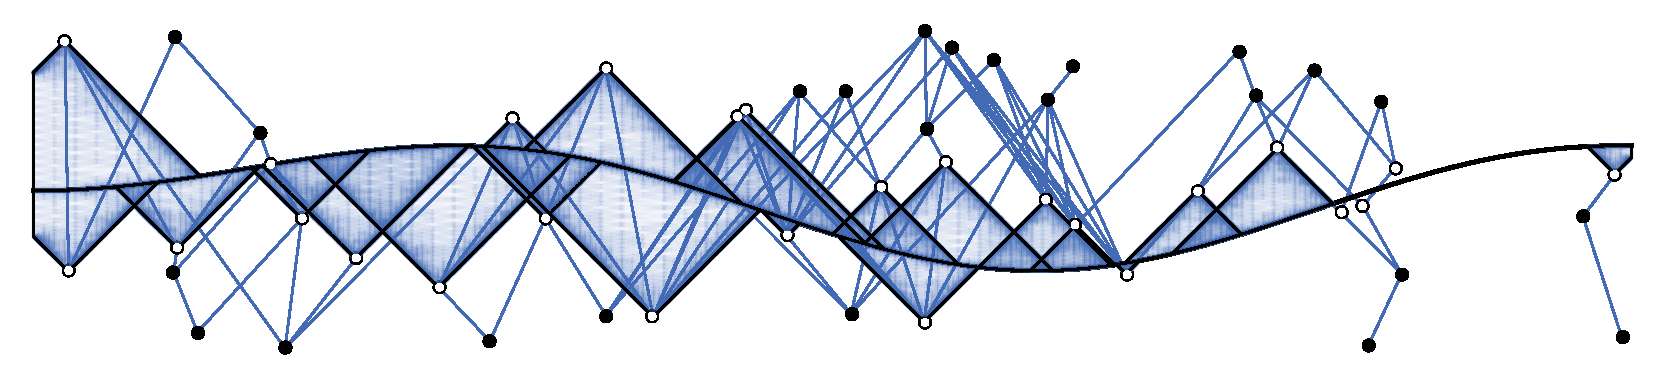
\includegraphics[width=\textwidth]{minmaxplot}
     \caption{An illustration of the idea. Pictured here is a causal set obtained by a sprinkling into a spacetime with a partitioning spacelike hypersurface. The minimal and maximal points about the surface are highlighted and the shaded regions illustrate the regions whose volumes are needed for the calculation.}
     \label{fig:Nmin_Nmax}
\end{figure}

\section{The Proof}

\subsection{Poisson Sprinklings for $\langle N_{max}\rangle$ and $\langle N_{min}\rangle$}

In order to prove~\eqref{eq:mainconjecture} let us choose a set of synchronous or Gaussian Normal Coordinates (GNC) adapted to $\Sigma$ such that in a neighbourhood $U_\Sigma$ of $\Sigma$ the line element is
\be
ds^2 = -dt^2 + h_{ij}(t,\mathbf x) dx^i dx^j.
\ee
In these coordinates, the surface $\Sigma$ corresponds to $t=0$, and the coordinate $t$ measures the proper time elapsed along geodesics whose tangent vector is proportional to the surface normal on $\Sigma$.
%\be\label{GNC_metric}
%g_{\mu\nu}(x)=
%\begin{pmatrix}
 %-1&0 \\
% 0&h_{ij}(x)
%\end{pmatrix}.
%\ee

%In order to find $N_{max}$, the number of maximal points below the surface, one has to use the fact that the points have been sprinkled with a Poisson distribution. 
For a sprinkling into $(M,g)$, the probability that a sprinkled point $x$ below the surface is \emph{maximal} is given by the probability that the sprinkling contains no points in the intersection $J^{+}(x)\cap J^{-}(\Sigma)$ of the causal future of $p$ with the causal past of the surface $\Sigma$. This region will in general be some sort of curvy $d$-dimensional cone. The Poisson distribution assigns a probability
\be\label{Poisson}
\mathbb P\left(\text{no points in }J^{+}(x)\cap J^{-}(\Sigma)\right)=e^{-\rho V(x,\Sigma)}
\ee
to this event, where $V(x,\Sigma):=V(J^{+}(x)\cap J^{-}(\Sigma))$ is the spacetime volume of the region $J^{+}(x)\bigcap J^{-}(\Sigma)$. The probability of sprinkling an element into an infinitesimal volume element $d^dx$ at $x\in M$ is $\rho\sqrt{-g(x)}d^dx$, where $\rho$ is the density of the sprinkling, and so the total expected number of maximal elements below $\Sigma$ is

\be\label{eq:nmax}
\left\langle N_{max}\right\rangle =\rho\int_{J^{-}(\Sigma)}d^{d}x\:\sqrt{-g}\\ e^{-\rho V(x,\Sigma)}
\ee

Similarly the expected number of minimal elements above $\Sigma$ is
\be\label{eq:nmin}
\left\langle N_{min}\right\rangle =\rho\int_{J^{+}(\Sigma)}d^{n}x\:\sqrt{-g}\ \ e^{-\rho V(\Sigma,x)}
\ee
where $V(\Sigma,x):=V(J^{+}(\Sigma)\cap J^{-}(x))$.

In the limit $\rho\rightarrow\infty$, both quantities will diverge, but if their difference $\langle N_{max}\rangle - \langle N_{min}\rangle = \langle N_{max} - N_{min}\rangle$ grows slower than or at order $\rho^{1-\frac2d}$, the proposed action~\eqref{GH_boundary_to_causet} will tend to a finite value in the continuum limit.

If we pick a point $x_0=(0,\mathbf{x})\in \Sigma$ on the surface that has the same spatial coordinates as $x=(t,\mathbf{x})$ then the coordinate time, $t$, is the proper time elapsed along the unique geodesic between $x_0$ and $x$. The volume $V(\Sigma,x)$ then only depends on $t$. Now as $\rho\rightarrow\infty$, we may pick any $\epsilon>0$ such that the contribution to \eqref{eq:nmax} and \eqref{eq:nmin} from points with $|t|>\epsilon$ will be negligible. We assume now that for large enough $\rho$, the region $\left\{|t|<\epsilon\right\}$ is entirely contained in the neighbourhood $U_\Sigma$ in which the GNC are valid.
Equations \eqref{eq:nmax} and \eqref{eq:nmin} can then be simplified as any time, $t$, which is far away from the surface will give rise to a large volume, which will then be exponentially suppressed as $\rho \rightarrow \infty$. More technically, if we choose some finite coordinate distance $\varepsilon$ away from the surface, either to the past or future, then any volume $V(p,\Sigma)$ or $V(\Sigma,q)$ with $|t|>\varepsilon$ will contribute nothing to the integral as $\rho \rightarrow \infty$. This $\varepsilon$ can be chosen arbitrarily close to $0$ allowing one to expand metric in $t$ about $t=0$. This gives

\begin{align}\label{eq:nmax_and_eq:nmin}
\left\langle N_{max}\right\rangle & =\int_{\Sigma}d^{d-1}x\int_{-\varepsilon}^{0}dt\:
h^{\frac{1}{2}}\left(1+
\frac{1}{2}\frac{\dot{h}}{h}t+O(t^2)\right)
 \rho\ e^{-\rho V(-t,\mathbf{x};0,\mathbf{x})}
\\
\left\langle N_{min}\right\rangle & =\int_{\Sigma}d^{d-1}x\int_{0}^{\varepsilon}dt\:
h^{\frac{1}{2}}\left(1+
\frac{1}{2}\frac{\dot{h}}{h}t+O(t^2)\right) \rho\ e^{-\rho V(0,\mathbf{x};t,\mathbf{x})}
\end{align}
where $h\equiv det\left(h_{ij}(0,\mathbf{x})\right)$ and $\dot{}\equiv \frac{\partial}{\partial t}$. The metric determinant has been in expanded in small $t$. The volume functions have been rewritten as follows: $V(x,\Sigma)=V(x,x_0)=V(-t,\mathbf{x};0,\mathbf{x})$ and $V(\Sigma,q)=V(x_0,x)=V(0,\mathbf{x};t,\mathbf{x})$

The only curvy cones that will contribute will have small volumes, as we are restricting ourselves close to the surface. This means that the volumes can be approximated by the volumes of less curvy cones, and it can be shown that higher order corrections, in the approximation scheme, vanish in the limit of $\rho \rightarrow \infty$. This will all be made more precise below. The approximation procedure will be outlined below for a cone to the future of $\Sigma$, as the process for the past cone is nearly identical. Riemann normal coordinates are integral to the following calculation so it is worth noting the relevant formulas before jumping in. 

\subsection{Riemann Normal Coordinates}

One can always find Riemann normal coordinates (RNC), about a point $p$, by changing from coordinates $x^{\alpha}$ to coordinates $y^{\overline{\alpha}}$ such that in these new coordinates the metric and the Christoffel symbols at $p$ are that of flat space. These conditions  can be expressed as follows

\be\label{eq:RNCMetricTransAtPAndChris}
g_{\overline{\alpha} \overline{\beta}}(p)=\eta_{\overline{\alpha} \overline{\beta}}=A^{\alpha}_{\;\overline{\alpha}}A^{\beta}_{\;\overline{\beta}}g_{\alpha\beta}(p)\;,\;\;\;\;\Gamma^{\overline{\alpha}}_{\;\overline{\beta}\overline{\gamma}}(p)=0
\ee
The $A^{\alpha}_{\;\overline{\alpha}}$ govern the coordinate transformation to linear order, but $O(x^2)$ corrections may be required. To second order the coordinate transformation is given by

\be\label{eq:RNCtotaltrans}
y^{\overline{\alpha}}=A^{\overline{\alpha}}_{\;\beta}x^\beta+\frac{1}{2}A^{\overline{\alpha}}_{\;\alpha}\Gamma^{\alpha}_{\;\beta\gamma}(p)x^\beta x^\gamma+O(x^3)
\ee
and the inverse transformation is just

\be\label{eq:RNCinversetrans}
x^{\alpha}=A^{\alpha}_{\;\overline{\beta}}y^{\overline{\beta}}+O(y^2)
\ee
One finds that the $A^{\alpha}_{\;\overline{\alpha}}$ also satisfy

\be\label{eq:RNCeqnforA}
A^{\overline{\alpha}}_{\;\mu}A^{\mu}_{\;\overline{\beta}}=\delta^{\overline{\alpha}}_{\;\overline{\beta}}\;,\;\;\;\;A^{\alpha}_{\;\overline{\mu}}A^{\overline{\mu}}_{\;\beta}=\delta^{\alpha}_{\;\beta}
\ee
These relations for RNC will cover all that will be needed in this discussion.

\subsection{Lightcone Volumes}

The volumes of the truncated lightcones can be found as follows. Consider the past lightcone emanating at the point $p_0=(T,\mathbf x_0)$. There is a unique point $q_0=(0,\mathbf x_0)$ on $\Sigma$ associated with $p_0$, separated from $p_0$ by a proper time $T$. 

The volume of this cone is given by

\be\label{eq:VolumeWithNoSimplifications}
V(0,\mathbf{x}_0;T,\mathbf{x}_0)=\int_{\mathcal{X}} d^d x\;\sqrt{-g}
\ee
where the integration region, $\mathcal{X}:= J^-(p_0)\bigcap J^+(\Sigma)$ will be some complicated thing. As we are dealing with points close to the surface we can use the  Riemann normal coordinates $y^{\overline{\mu}}$, defined as above, about the point $q_0$ (the point $q_0$ being the origin of our RNC system). One finds that $A^0_{\;\overline{0}}=1$, $A^0_{\;i}=0$ and $\delta_{\overline{\emph\i}\overline{\emph\j}}=A^i_{\;\overline{\emph\i}}A^j_{\;\overline{\emph\j}}h_{ij}(0,\mathbf{x}_0)$. It can be shown that the volume integral reduces to \cite{Khetrapal_Sumati:Causal_Diamond_Volume}

\be\label{eq:VolumeWithRNC}
V(0,\mathbf{x}_0;T,\mathbf{x}_0) =\int_{\mathcal{X}}d^dy+\int_{\mathcal{X}_0}d^dy\left(-\frac{1}{6}R_{\overline{\mu}\overline{\nu}}(q_0)y^{\overline{\mu}}y^{\overline{\nu}} \right)+O(T^{d+3})
\ee
where $\mathcal{X}_0=\left\lbrace y^{\overline{\mu}} \mid 0\leq y^{\overline{0}}=\overline{t}\leq T\; ,\; \sqrt{(y^{\overline{1}})^2+(y^{\overline{2}})^2+...+(y^{\overline{d-1}})^2}\leq T-\overline{t} \right\rbrace$ is what we call the \textit{flat cone}, and $R_{\overline{\mu}\overline{\nu}}(q_0)$ is the Ricci tensor in RNC evaluated at $q_0$. The arguments of the volume function need not be changed as the volume only depends on the points in the manifold, $q_0$ and $p_0$. The \textit{flat cone} term comes in at $O(T^{d+2})$ so the volume we have to calculate has reduced to

\be\label{eq:VolumeToLowestOrder}
V(0,\mathbf{x}_0;T,\mathbf{x}_0) =\int_{\mathcal{X}}d^dy+O(T^{d+2})
\ee
Terms of $O(T^{d+2})$ can be retained till the end, but in the limit, $\rho\rightarrow\infty$, they vanish. This will be proved below.

The boundaries of $\mathcal{X}$ must now be figured out in order to do this integral. First we look at the top part of the cone. From \cite{Khetrapal_Sumati:Causal_Diamond_Volume} it can be shown that the first curvature correction to the top part of the cone comes in at $O(T^{d+2})$ and so can be ignored for our purposes. This means that the top can be treated as a that of a \textit{flat cone} and so points on the boundary obey the equation $\sqrt{(y^{\overline{1}})^2+(y^{\overline{2}})^2+...+(y^{\overline{d-1}})} = T-\overline{t}$.

The bottom surface of the cone was defined in terms of GNC to be $t=0$, so we can use (\ref{eq:RNCtotaltrans}) to find the equation for the surface in RNC. Equation (\ref{eq:RNCtotaltrans}) gives

\be\label{eq:BottomSurfaceWithGNC}
y^{\overline{0}}=\overline{t}=\frac{1}{2}\Gamma^{0}_{\;ij}(0,\mathbf{x}_0)x^i x^j+O(x^3)
\ee
The first part on the right of (\ref{eq:RNCtotaltrans}) vanishes as $A^{\overline{0}}_{\;\mu}x^{\mu}=x^0$ (as $A^{\overline{0}}_{\;i}=0$ and $A^{\overline{0}}_{\;0}=1$) and $x^0=t=0$ for the bottom surface. Using the inverse RNC relation (\ref{eq:RNCinversetrans}) one can find the equation for the bottom surface entirely in RNC.

\be\label{eq:BottomSurface}
\overline{t}=\frac{1}{2}\Gamma^{0}_{\;ij}(0,\mathbf{x}_0)A^{i}_{\;\overline{\emph\i}}A^{j}_{\;\overline{\emph\j}}y^{\overline{\emph\i}} y^{\overline{\emph\j}}+O(y^3)
\ee

This equation can be written in terms of the radial coordinate of the cone, $r=\sqrt{(y^{\overline{1}})^2+...+(y^{\overline{d-1}})^2}$, as

\be\label{eq:RadialBottomSurface}
\overline{t}=\frac{1}{2}\left(\Gamma^{0}_{\;ij}(0,\mathbf{x}_0)A^{i}_{\;\overline{\emph\i}}A^{j}_{\;\overline{\emph\j}}\frac{y^{\overline{\emph\i}} y^{\overline{\emph\j}}}{r^2}\right)r^2+O(y^3)=\frac{1}{2}f(\mathbf{x}_0,\phi)r^2+O(y^3)
\ee
where $\phi$ stands for all the angular coordinates $\phi_1,..,\phi_{d-2}$. The function $f(\mathbf{x}_0,\phi)$ depends on $\mathbf{x}_0$ as $\Gamma^{0}_{\;ij}$ and $A^{i}_{\;\overline{\emph\i}}$ will, in general, be different for a different point on the surface. One can see that $f(\mathbf{x}_0,\phi)$ depends on the angles, $\phi$, by substituting the relations below into (\ref{eq:RadialBottomSurface})

\begin{equation}
\begin{aligned}\label{eq:SphericalCoords}
y^{\overline{1}} &= r \cos(\phi_1)  \\
y^{\overline{2}} &= r \sin(\phi_1) \cos(\phi_2)  \\
y^{\overline{2}} &= r \sin(\phi_1) \sin(\phi_2) \cos(\phi_3)  \\
    &\vdots  \\
y^{\overline{d-2}} &= r \sin(\phi_1) \cdots \sin(\phi_{d-3}) \cos(\phi_{d-2})  \\
y^{\overline{d-1}} &= r \sin(\phi_1) \cdots \sin(\phi_{d-3}) \sin(\phi_{d-2})
\end{aligned}
\end{equation}

With the boundaries of the integration region in place, we can now write down the integral explicitly, in spherical coordinates:

\be\label{eq:VolumeIntegralSpherical}
V(0,\mathbf{x}_0;T,\mathbf{x}_0)=\int_{S^{d-2}}
d\Omega_{d-2}
\int_{0}^{r_{max}(\phi)}r^{d-2}dr
\int_{\frac{1}{2}f(\mathbf{x}_0,\phi)r^2}^{-r+T}
d\overline{t}+O(T^{d+2})
\ee
where $r_{max}(\phi)$ is the radial coordinate of where the bottom surface meets the top part of the cone at an angle $\phi$, shown in \ref{fig:cone_plot}. To find this one needs to solve $\frac{1}{2}f(\mathbf{x}_0,\phi){r_{max}}^2(\phi)=-r_{max}(\phi)+T$ and take the positive solution. The solution can be expanded in $T$ and is simply $r_{max}=T+O(T^2)$, with angular dependent terms contributing at $O(T^2)$. The $O(T^2)$ term will contribute at $O(T^{d+2})$ in the integral and so can be ignored. Substituting $r_{max}=T$ into (\ref{eq:VolumeIntegralSpherical}) means it can be evaluated to give
\begin{figure}[t]
  \centering
    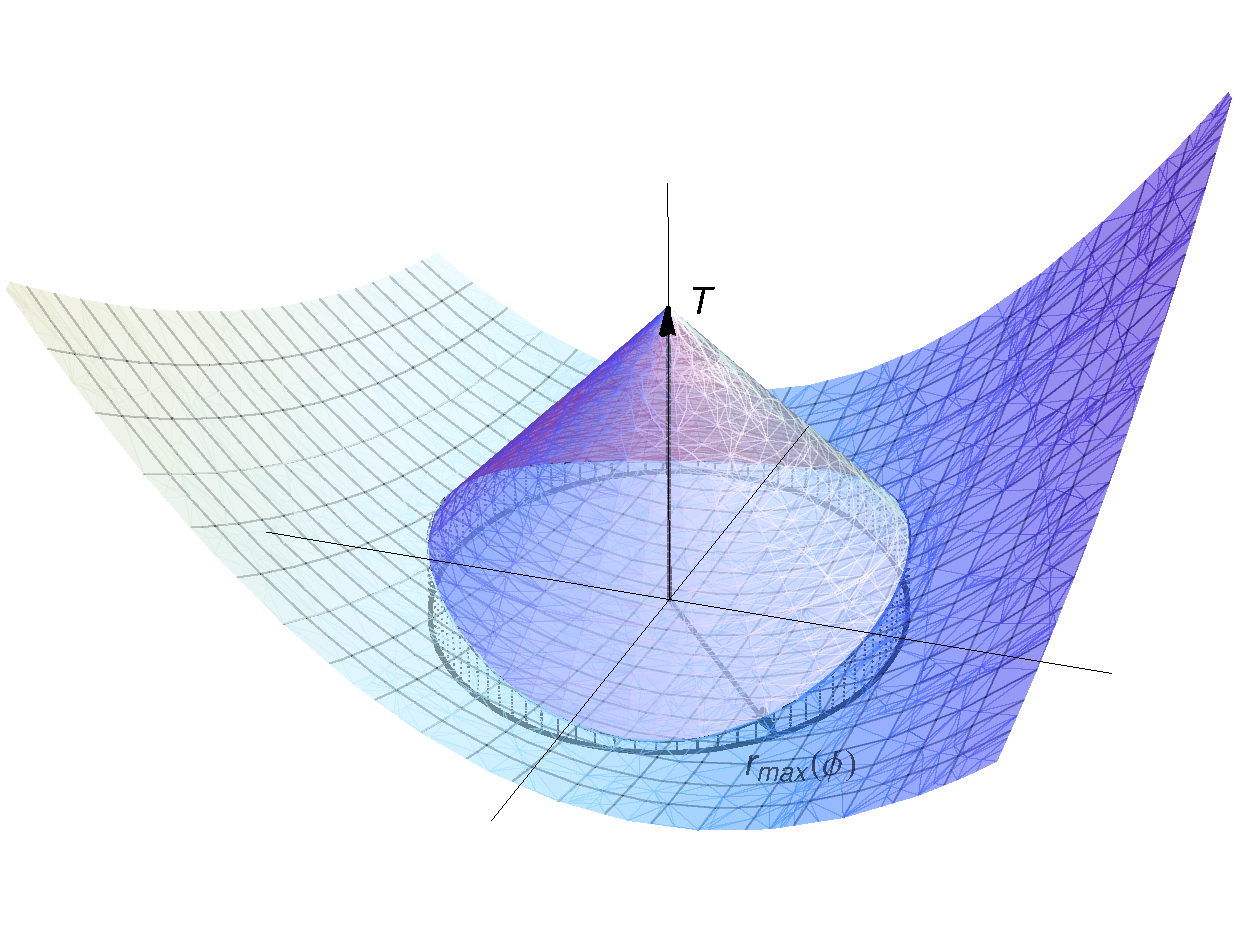
\includegraphics[scale=0.5]{coneplot}
     \caption{The size of the region inside the top and bottom bounding surfaces is the volume we want to calculate.}
     \label{fig:cone_plot}
\end{figure}
\be\label{eq:VolumeNoK}
V(0,\mathbf{x}_0;T,\mathbf{x}_0)
=\frac{A_{d-2}}{d(d-1)}T^d\left(1-\frac{d}{2(d+1)}\Gamma^{0}_{\;ij}(0,\mathbf{x}_0)A^{i}_{\;\overline{\emph\i}}A^{j}_{\;\overline{\emph\j}}\delta^{\overline{\emph\i}\overline{\emph\j}}T\right)
+O(T^{d+2})
\ee
where $A_{d-2}$ is the $d$-$2$ dimensional volume of a $d$-$2$ dimensional sphere and the $\delta^{\overline{\emph\i}\overline{\emph\j}}$ has come from the fact that cross terms ($\overline{\emph\i}\neq \overline{\emph\j}$) vanish under the angular integration. The defining relations for $A^{i}_{\;\overline{\emph\i}}$ can be rearranged to give $A^{i}_{\;\overline{\emph\i}}A^{j}_{\;\overline{\emph\j}}\delta^{\overline{\emph\i}\overline{\emph\j}}=h^{ij}(0,\mathbf{x}_0)$. In GNC it can be shown that the extrinsic curvature is given by

\be\label{eq:K}
K(0,\mathbf{x}_0)
=g^{\mu\nu }\nabla_{\mu}n_{\nu}
=-\Gamma^{0}_{\;ij}(0,\mathbf{x}_0)h^{ij}(0,\mathbf{x}_0)=-\frac{1}{2}\frac{\dot{h}(0,\mathbf{x}_0)}{h(0,\mathbf{x}_0)}
\ee
which means that the first correction to the volume of the cone depends on $K(0,\mathbf{x}_0)$, and thus the approximate volume of the cone is

\begin{align}
V(0,\mathbf{x}_0;T,\mathbf{x}_0)
&=\frac{A_{d-2}}{d(d-1)}T^d\left(1+\frac{d}{2(d+1)}K(0,\mathbf{x}_0)T\right)
+O(T^{d+2}) \label{eq:TopVolumeWithK}\\
V(-T,\mathbf{x}_0;0,\mathbf{x}_0)
&=\frac{A_{d-2}}{d(d-1)}T^d\left(1-\frac{d}{2(d+1)}K(0,\mathbf{x}_0)T\right)
+O(T^{d+2}) \label{eq:BottomVolumeWithK}
\end{align}
where (\ref{eq:BottomVolumeWithK}) is the volume of the cone with its tip below the surface, and can be found from similar arguments.

\subsection{Final Stretch of the Proof}

Let us now use these volume functions in the expressions for $\left\langle N_{max}\right\rangle$ and $\left\langle N_{min}\right\rangle$ to calculate the $\left\langle N_{max}-N_{min}\right\rangle$ term in equation (\ref{GH_boundary_to_causet}) as $\rho \rightarrow \infty$. We have
\begin{gather}\label{eq:NmaxNminStart}
\begin{aligned}
\lim_{\rho \to \infty}\rho^{\frac{2}{d}-1}\left\langle N_{max}-N_{min} \right\rangle &= \\
\lim_{\rho \to \infty}\rho^{\frac{2}{d}}
\int_{\Sigma}d^{d-1}x & \int_{-\varepsilon}^{0}dt\
h^{\frac{1}{2}}\left(1+
\frac{1}{2}\frac{\dot{h}}{h}t-\rho B(-1)^{d}t^{d+1}+\rho O(t^{d+2})\right)e^{-\rho A(-1)^{d}t^{d}} \\
-\rho^{\frac{2}{d}}\int_{\Sigma}d^{d-1}x &
\int_{0}^{\varepsilon}dt\
h^{\frac{1}{2}}\left(1+
\frac{1}{2}\frac{\dot{h}}{h}t-\rho Bt^{d+1}+\rho O(t^{d+2})\right)e^{-\rho At^{d}}
\end{aligned}
\end{gather}
where we have defined
\begin{gather}\label{A_and_B_defn}
\begin{aligned}
A & \equiv \frac{A_{d-2}}{d(d-1)} \\
B & \equiv \frac{A_{d-2}}{2(d-1)(d+1)}K(0,\mathbf{x})
\end{aligned}
\end{gather}
and we have Taylor expanded the $O(t^{d+1})$ parts of the volume functions, in small $t$, from the exponents. We have also included a pre-factor of $\rho^{\frac{2}{d}-1}$ to account for the factors of $l$ in (\ref{GH_boundary_to_causet}). With this pre-factor the limit of the above equation is well defined. If we change to $u=-t$ in the first part on the right hand side, and $u=t$ on the second part then the integral can be simplified to
\be\label{eq:NmaxNminSimplified}
\lim_{\rho \to \infty}\rho^{\frac{2}{d}}
\int_{\Sigma}d^{d-1}x \int_{0}^{\varepsilon}du\
h^{\frac{1}{2}}\left(-\frac{\dot{h}}{h}u+2\rho B u^{d+1}+\rho O(u^{d+2}) \right)e^{-\rho Au^{d}}
\ee
We now show that $O(u^{d+2})$, or higher, terms vanish as $\rho \rightarrow\infty$. All higher order corrections that we have ignored so far contribute at $O(u^{d+2})$ or higher, so proving that these contributions vanish proves that our approximations are valid. Taking only the part we are interested in from (\ref{eq:NmaxNminSimplified}) leaves us with the task of showing that the following integral vanishes.

\be\label{eq:VanishingOrderIntegral}
\lim_{\rho \to \infty}\rho^{\frac{2}{d}+1}\int_{0}^{\varepsilon}du\
u^{d+n}e^{-\rho Au^{d}}
\ee
for $n>1$, where $n\in\mathbb{N}$. The additional factor of $\rho$ has come from inside the integral in (\ref{eq:NmaxNminSimplified}). We make the substitution $z=\rho Au^{d}$ and find that (\ref{eq:VanishingOrderIntegral}) is proportional to

\be\label{eq:GammaVanishingOrderIntegral}
\lim_{\rho \to \infty}\rho^{\frac{1-n}{d}}\int_{0}^{\rho A\varepsilon^d}dz\;z^{\frac{n+1}{d}}e^{-z}=\lim_{\rho \to \infty}\rho^{\frac{1-n}{d}}\int_{0}^{\infty}dz\;z^{\left[\left(\frac{n+1}{d}+1\right)-1 \right]}e^{-z}
\ee
where $\rho$ has been taken to $\infty$ in the limits on the RHS, and the power of $z$ has been written in this way so that the integral is in the form of a gamma function, $\Gamma(t)=\int_{0}^{\infty}z^{t-1}e^{-z}dz$. Using the fact that for gamma functions, $\Gamma(t+1)=t\Gamma(t)$, we find that (\ref{eq:GammaVanishingOrderIntegral}) is then proportional to

\be\label{eq:GammaVanishingOrder}
\lim_{\rho \to \infty}\rho^{\frac{1-n}{d}}\Gamma\left(\frac{n+1}{d}\right)
\ee
One can see from above that if $n>1$ then this term will vanish, thus proving that terms of $O(u^{d+2})$ or higher will go to $0$ in the limit $\rho\rightarrow\infty$.

The non-vanishing terms of (\ref{eq:NmaxNminSimplified}) can also be put into the form of gamma functions. This allows the integral over $u$ to be evaluated in (\ref{eq:NmaxNminSimplified}). One also sees that we have terms like $\frac{\dot{h}}{h}$, and from (\ref{eq:K}) we know that these can be written in terms of the extrinsic curvature, $K(0,\mathbf{x})$. We find then that (\ref{eq:NmaxNminSimplified}) reduces to

\be\label{eq:nmax_eq:nmin_end}
\lim_{\rho \to \infty}\rho^{\frac{2}{d}-1}\left\langle N_{max}-N_{min} \right\rangle=
\frac{2(d+2)}{d(d+1)}
\left[\frac{A_{d-2}}{d(d-1)}\right]^{-\frac{2}{d}}
\Gamma\left(\frac{2}{d}\right)\int_{\Sigma}d^{d-1}x\
\sqrt{h}K(0,\mathbf{x}).
\ee
$K(0,\mathbf{x})$ is evaluated at the surface and is therefore the same $K$ as in equation (\ref{GH_boundary_to_causet}). We can therefore conclude that to make (\ref{eq:mainconjecture}) true we need a factor $l_{p}^{2-d}$ to make our expression dimensionless, and a value of $c_d$ equal to that of equation (\ref{Cn}). This concludes the proof of the conjectured equality in (\ref{eq:mainconjecture}).

\section{Fluctuations}
So far we have only talked about the mean of the causal set boundary action. Let us now turn to its fluctuations (the standard deviation) $\sigma[S^{(d)}_{GHY}(\mathcal C)]=\text{Var}[S^{(d)}_{GHY}(\mathcal C)]^\frac12$.\footnote{Whenever we say fluctuations we refer to the standard deviation of the random variable, not to its variance.} We can make a heuristic argument to estimate the dependence of fluctuations on $\rho$. In any spacetime region of fixed volume $V$ the number of causal set elements $N$ experiences Poisson fluctuations of order $\sqrt N$. Since $N_{max}$ and $N_{min}$ are quantities associated with a codimension-1 surface (counting elements ``near" $\Sigma$), we may expect them to inherit fluctuations of order $N^\frac{d-1}{2d}$. Then the action $S^{(d)}_{GHY}$, being proportional to $\rho^\frac{d-2}{d}$ times the difference of two independent\footnote{The independence is as a feature of the Poisson process in $M$: the number of elements $N(R)$ in any subregion $R\subset M$ is a Poisson variable itself, and for any two disjoint regions $R_1$, $R_2$ the numbers $N(R_1)$ and $N(R_2)$ are independent random variables.} random variables with standard deviation $N^\frac{d-1}{2d} = (\rho V)^\frac{d-1}{2d}$ should see fluctuations of order $\rho^\frac{2-d}{d}\rho^\frac{d-1}{2d}=\rho^\frac{d-3}{2d}$. This suggests that for $d=2$ these fluctuations should grow as $\rho\rightarrow\infty$, for $d=3$ they should be constant, and for $d>3$ they should be damped.

In order to test this heuristic argument one may like to write down the integral expression for $\text{Var}[S^{(d)}_{GHY}(\mathcal C)]^\frac12$ but it is complicated enough even in finite regions of flat space that it is not very illuminating to reproduce it here. Instead we will show the results of computer simulations that support results of the heuristic argument. 
 
The simulations were carried out as follows. Denote the discreteness scale by $l$. Take a $d$-cube $[0,L]^d$ in $d$-dimensional Minkowski space with metric $ds^2=-dt^2+d{\mathbf x}^2$ and define the hypersurface $\Sigma: t=L/2$, which partitions the cube into two halves. Sprinkle at density $\rho=l^{-d}$ into the cube, which in any given run will place $N$ points inside the cube where $N$ is a Poisson random number with mean $\left\langle N\right\rangle = \rho V=  (L/l)^d$. Evaluate $S^{(d)}_{GHY}=c_d\rho^\frac{d-2}{d}(N_{min} - N_{max})$ for $\Sigma$ by counting the minimal/maximal elements in the upper/lower half of the cube, and repeat.

\bibliographystyle{utphys}

\bibliography{references}{}

\end{document}


%%
JHEPPUB:

\title{Gibbons-Hawking-York Boundary Term in Causal Sets}
 \author[a]{M. Buck}
 \author[a,b]{\!, F. Dowker}
 \author[a]{and I. Jubb\,}
\affiliation[a]{Theoretical Physics Group, Blackett Laboratory, Imperial College, London, SW7 2AZ, U.K.}
\affiliation[b]{Institute for Quantum Computing, University of Waterloo, ON, N2L 2Y5, Canada}

\abstract{ 
We show some stuff.
}

\begin{document}

\maketitle

\pagebreak

\noindent NOTES:\\
1. define s as the RV, not as its mean

\section{Introduction}




%%IOPART

\begin{document}

\title{Gibbons-Hawking-York Boundary Term in Causal Sets}

\author{Michel Buck Fay Dowker, Ian Jubb}
\address{Blackett Laboratory, Imperial College, London, SW7 2AZ, U.K.}

\begin{abstract}

We show some stuff.

\end{abstract}
%\pacs{03.67.-a, 03.65.Ta, 03.70.+k}

\maketitle
\section{Introduction}
%%